
\subsubsection{Experiential Learning in an XR environment}

Experiential learning theory posits that learning is a process through which knowledge is created via the transformation of experience \parencite{kolb1984}. This perspective emphasizes that learning emerges through the integration of experiencing, reflecting, thinking, and acting within a continuous cycle.

Kolb conceptualizes learning as a four-stage cyclical process consisting of concrete experience (CE), reflective observation (RO), abstract conceptualization (AC), and active experimentation (AE) \parencite{almeida_learning_2010}, as illustrated in \cref{fig:exp4stages}.

Concrete experience refers to the learner's direct engagement in a specific activity, where immersive technologies such as extended reality (XR) can enhance the sense of presence. Reflective observation involves consciously reflecting on the experience, often supported by feedback mechanisms or guidance;in this context, a human-AI collaboration agent can provide timely and accurate support to help learners interpret their experiences. Abstract conceptualization entails the formation or refinement of theoretical constructs and hypotheses derived from reflection. Finally, active experimentation involves applying these conceptualizations to new situations, allowing learners to test their understanding and generate new experiences, thereby continuing the learning cycle.


\begin{figure}[H]
\caption{The Four-Stage Learning Cycle by Kolb (1984)}\label{fig:exp4stages}
\centering
\centering
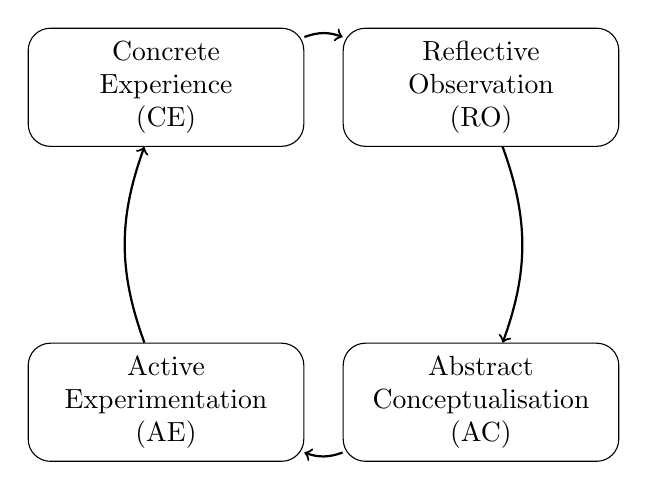
\begin{tikzpicture}[
    node distance=4cm,
    every node/.style={
        draw,
        rounded corners=8pt,
        minimum width=3.5cm,
        minimum height=1.5cm,
        align=center
    },
    arrow/.style={->, thick}
]

% Nodes
\node (ce) {Concrete\\Experience\\(CE)};
\node (ro) [right of=ce] {Reflective\\Observation\\(RO)};
\node (ac) [below of=ro] {Abstract\\Conceptualisation\\(AC)};
\node (ae) [left of=ac] {Active\\Experimentation\\(AE)};

% Arrows
\draw[arrow] (ce) to[bend left=20] (ro);
\draw[arrow] (ro) to[bend left=20] (ac);
\draw[arrow] (ac) to[bend left=20] (ae);
\draw[arrow] (ae) to[bend left=20] (ce);

\end{tikzpicture}
\end{figure}


Prior research suggests that virtual reality (VR), as an experiential learning tool, can effectively enhance technical skills and learner confidence, even with relatively short exposure times \parencite{knobovitch_virtual_2025}. VR also enables personalized learning experiences by allowing students to explore virtual environments at their own pace and according to their individual preferences. Furthermore, VR systems can support improved comprehension through the delivery of adaptive and personalized feedback \parencite{marougkas_virtual_2023}.

In addition, the immersive and interactive nature of XR has been shown to promote higher levels of engagement, both physically and cognitively \parencite{liu_research_2025}. Compared with flat display devices, XR-based approaches can also improve learner concentration. For example, \textcite{liu_research_2025} found that learners in a VR-based instruction (VRI) group demonstrated higher task mastery rates than those in other groups. This improvement was attributed to increased engagement and interactivity, which supported better information retention.